%
% Perfil histórico
%
\chapter{Perfil histórico}
\addcontentsline{lof}{chapter}{1. Perfil histórico}

El presente trabajo estudia la función gamma de Euler desde su primera representación, la cual fue hecha por el matemático suizo Leonhard Euler (1707-1783), en una carta escrita el 13 de octubre de 1729 al matemático prusiano Christian Goldbach (1690-1764). Esta carta fue la primera de muchas que conformaron una considerable correspondencia, que abarcaría desde el análisis hasta la teoría de números. Este breve perfil histórico está apoyado en Davis (1959), y los detalles respectivos a la deducción del producto infinito de Euler provienen de Andrews (1999). Como preámbulo se presentan los números triangulares, los cuales son una introducción amigable al problema de interpolación propuesto por Daniel Bernoulli (1700-1782) y Christian Goldbach al principio del siglo XVIII.

\section{Preámbulo}

A comienzos del siglo XVIII de la era cristiana, los matemáticos Daniel Bernoulli y Christian Goldbach enunciaron un problema abierto muy interesante que consistía en encontrar una fórmula analítica, que conste de solo operaciones básicas, de la fórmula factorial $$n! = 1\times 2\times 3 \times \dots \times n \ \textrm{donde} \ n\in\mathbb{N},$$
y que tal fórmula fuera válida para términos que no fueran números naturales.

Un problema parecido sería encontrar una expresión analítica de cierta sucesión numérica que interpole los términos de dicha sucesión tomando números diferentes a los números naturales. Si se toma por ejemplo, los números triangulares, es posible encontrar dicha expresión que cumpla con lo anterior.

Los números triangulares son aquellos que surgen del ordenamiento de puntos en triángulos equiláteros. Posiblemente los pitagóricos fueron los primeros en trabajar con este tipo de números, junto con otros "números figurados". Tal era la importancia que tenía este tipo de números en los pitagóricos, que el cuarto número triangular se consideraba un símbolo místico denominado el \textit{tetraktys}. Los números triangulares se pueden representar como en la Figura \ref{fig1_1}

\begin{figure}[htbp]
	\begin{center}
		\includegraphics[scale=0.5]{NumTriang.JPG}
	\end{center}
\caption{Números triangulares.}
\label{fig1_1}
\end{figure}

Por convención, el primer número pitagórico es el $1$. Los demás números se forman sumando al anterior el correspondiente número natural que simboliza su posición en la progresión. Así tenemos $$1,\ 1+2 = 3,\ 3+3 = 6,\ 6+4 = 10,\ 10+5=15,\ \dots$$

La progresión anterior conduce a la siguiente fórmula, $$T_n = 1+2+3+\dots+n = \frac{n(n+1)}{2},$$
que representaría al $n$-ésimo número triangular. 
Dicha fórmula está relacionada con la leyenda de Carl Friedrich Gauss. Se dice que Gauss dedujo esta fórmula a la edad de seis años, cuando su maestro les pidió a él y a sus compañeros de clase sumar todos los números naturales del $1$ al $100$. Después de un corto tiempo, el pequeño Gauss presentó el resultado correcto, Göllmann (2017).
Tal resultado era $5050$, la suma de los primeros $100$ números naturales, $$\sum_{k=1}^{100} \ k = 5050.$$

Si denotamos la suma de los primeros $n$ números naturales como $$S = \sum_{k=1}^{n}\ k,$$ entonces podremos llegar a
\begin{align*}
	2S &= \sum_{k=1}^{n} k + \sum_{k=1}^{n} (n+1-k)\\
	&= \sum_{k=1}^{n} (k+n+1-k)\\
	&= \sum_{k=1}^n (n+1)\\
	&= (n+1) \sum_{k=1}^n 1\\
	&= (n+1) n\\
\intertext{y así,}
 S &= \frac{n(n+1)}{2}.
\end{align*}
Por lo tanto, la fórmula para el $n$-ésimo número triangular ya queda demostrada.

Regresando al problema de Goldbach y Bernoulli, se requiere llegar a una fórmula parecida que solo necesite el conocimiento de $n$ y que además, solo se usen operaciones básicas. La sucesión numérica, $$1,\ 1\times2=2,\ 2\times3=6,\ 6\times4 = 24,\ \dots$$ es similar a la de los números triangulares, pero crece aún más debido a que sus términos se generan por productos. Este crecimiento tan pronunciado llamó la atención del matemático escocés James Stirling (1692-1770), que con varios intentos utilizando aproximaciones de $\ln n!$ no pudo llegar a la fórmula requerida, pero gracias a ello, dio un avance muy importante en lo que hoy se conoce como la fórmula de aproximación de Stirling.

Además, tal fórmula tiene que ser válida para valores que no sean números naturales, en otras palabras, ¿se podría encontrar la expresión factorial de una fracción? Por ejemplo, en el caso de los números triangulares, $T_{5\frac{1}{2}} = 17\frac{7}{8}$ se encuentra entre $T_5 = 15$ y $T_6 = 21$. Así, conociendo la tendencia creciente de la fórmula, se puede interpolar entre 2 números triangulares. ¿Será posible que suceda algo semejante con los términos factoriales?

En la Figura \ref{fig1_2} se muestra cómo la fórmula 
\begin{equation}
	T(x) = \frac{x(x+1)}{2}\ \textrm{para}\ x\in\mathbb{R},
\end{equation}
puede interpolar los valores de la sucesión de números triangulares. En la Figura \ref{fig1_3} vemos representados los números factoriales.
\begin{figure}[htbp]
	\begin{center}
		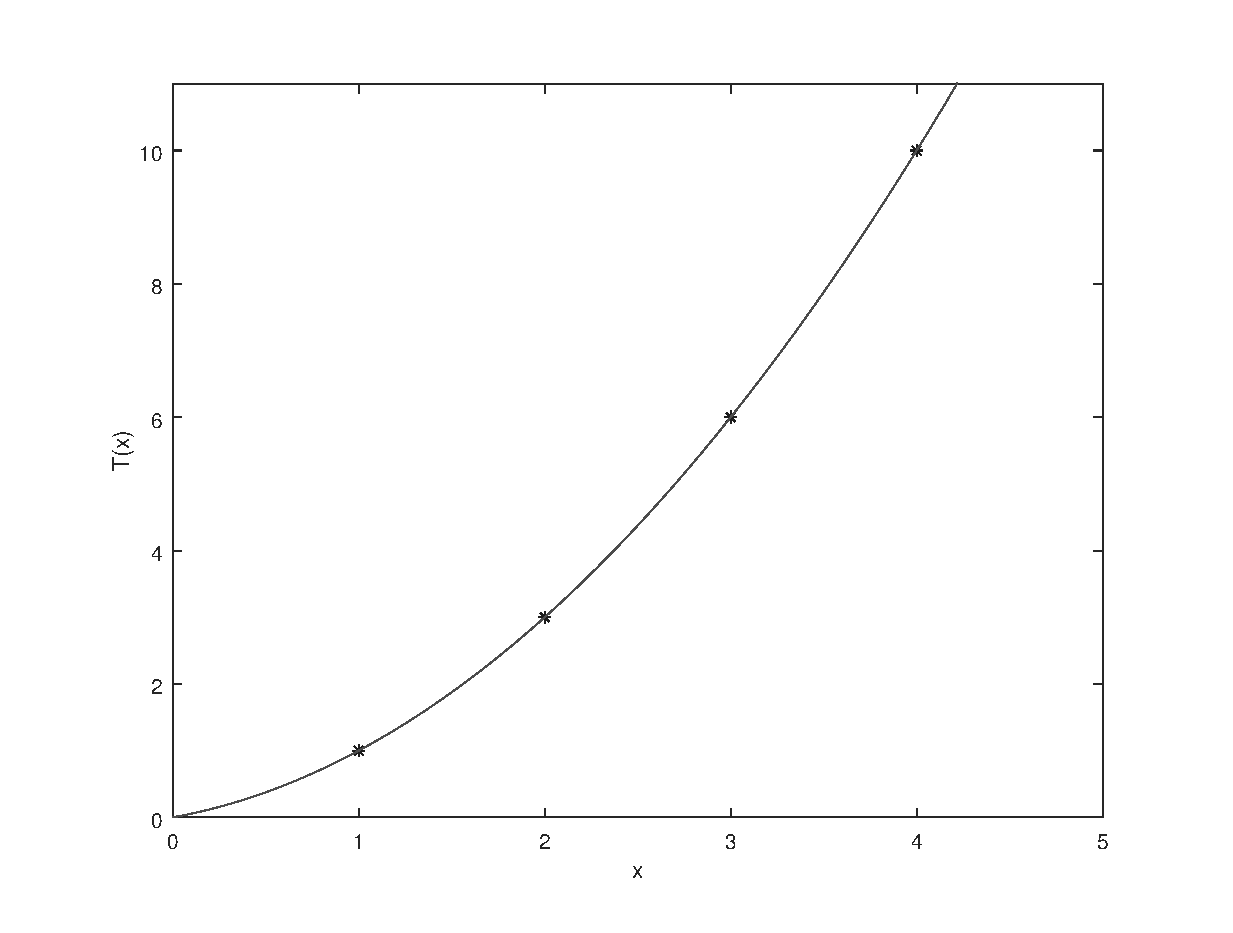
\includegraphics[scale=0.5]{figura1_2.eps}
	\end{center}
\caption{Interpolación de los números triangulares}
\label{fig1_2}
\end{figure}
\begin{figure}[htbp]
	\begin{center}
		\includegraphics[scale=0.5]{figura1_3.eps}
	\end{center}
\caption{Secuencia de números factoriales}
\label{fig1_3}
\end{figure}

Ahora, para iniciar con el estudio de la función gamma, se define de una manera formal la función factorial.
\begin{definition}
	Sea $n \in \mathbb{N}$, entonces la función factorial se define como $$n! = \prod_{k=1}^{n} k.$$
\end{definition}

Determinando así que $n!$ es el producto de los $n$ primeros números naturales. ¿Qué pasa con $0!$? Si volvemos a nuestros números triangulares, vemos que se cumple esta relación de recurrencia $$T_{n+1} = T_n + (n+1).$$ Si hacemos $n = 0$, obtenemos que $T_0 = 0.$ Así, $0$ sería un tipo de número triangular y esto, nos conlleva a la definición de suma vacía y producto vacío. 

\begin{definition}
		Sea $K$ un cuerpo y sean $a_k \in K$ con $k = 1,\ 2,\ 3,\ \dots,\ n$. Entonces para el conjunto $\{k \in \mathbb{N}\ :\ k\leq n\}$, $$\sum_{k>n} a_k = 0, \hspace{1cm} \prod_{k>n} a_k = 1.$$
\end{definition}

Lo anterior es resultado de que si $S_n = \sum_{k=1}^{n} a_k$ y $P_n = \prod_{k=1}^{n} a_k$ con $n \in \mathbb{N},$ entonces
$$S_{n+1} = a_{n+1}+S_n, \hspace{1cm} P_{n+1} = a_{n+1}P_n.$$
Como $S_1 = a_1$ y $P_1 = a_1$, podemos usar las expresiones anteriores con $n = 0$ y llegar a $S_0 = 0$ y $P_0 = 1,$ que corresponden a los elementos neutros de la suma y el producto del cuerpo. Luego, usando la definición 1.1, $0! = 1.$ Además, como $$n! = n \prod_{k=1}^{n-1} k,$$ entonces se llega a la fórmula de recurrencia del factorial
\begin{equation}
	n! = \left\{ \begin{array}{rcl}
	n(n-1)! & \mbox{para} & n\geq1\\
	&				&\\
	1 & \mbox{para} & n = 0.\\
	\end{array}\right.
\end{equation}

\section{El nacimiento de la función gamma de Euler}

En la sección anterior vimos que para la secuencia de números triangulares, se puede encontrar una fórmula general que funcione para todo $x \in \mathbb{R}$, la cual, cuando $x = n \in \mathbb{N}$, genere el $n$-ésimo número triangular correspondiente. Para la secuencia de números factoriales, Euler encontró que la fórmula
\begin{equation}
	n! = \int_{0}^{1}\, (-\ln t)^n\, dt, 
\end{equation}
genera valores numéricos para números diferentes a los enteros no negativos y, para el caso en que $n \in \mathbb{Z}_0^+,$ genera los números factoriales. En la Figura \ref{fig1_4} vemos cómo la fórmula (1.3) interpola los términos factoriales. 

Cabe destacar, que la fórmula (1.1) solo me genera números triangulares cuando $x = n \in\mathbb{N},$ porque para valores distintos pierde su significado original. Igualmente sucede con los números factoriales y la expresión (1.3), ya que $(1/2)!$ no es una expresión factorial. De hecho, encontramos extensiones de tales expresiones en $\mathbb{R}$, que al restringir su dominio a $\mathbb{Z}_0^+$ me generan números triangulares y factoriales respectivamente. De manera similar sucede con la suma infinita de todos los números naturales $$\sum_{k=1}^{\infty}\ k = -\frac{1}{12},$$ que se encuentra en Berndt (1985). Esta identidad no es completamente cierta, ya que la parte izquierda de la igualdad es una serie divergente, pero representa un hecho muy interesante relacionado con la función zeta de Riemann. Este resultado se explica con más detalle en el capítulo 4 del presente trabajo. 

\begin{figure}[htbp]
	\begin{center}
		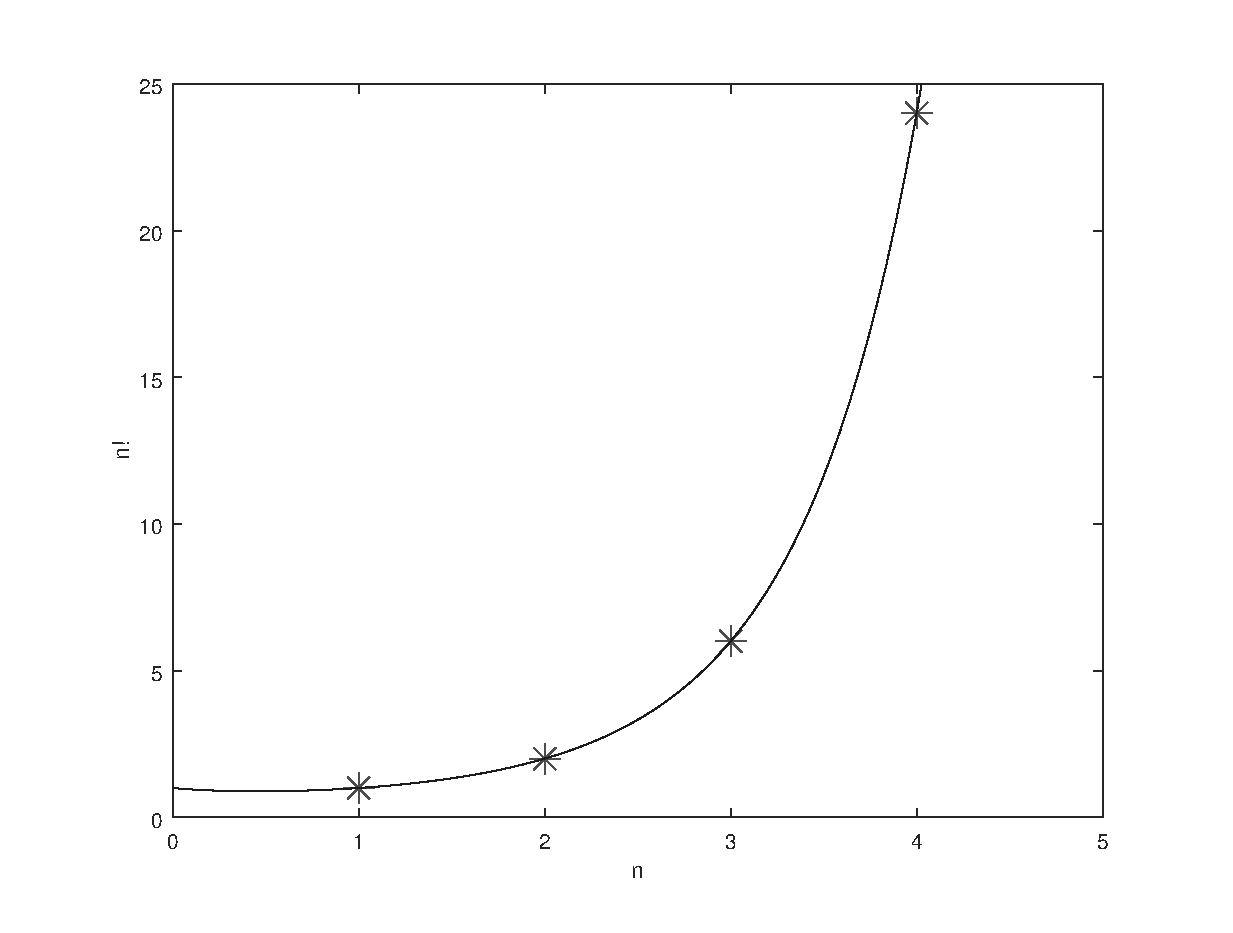
\includegraphics[scale=0.5]{figura1_4.eps}
	\end{center}
\caption{Interpolación de los números factoriales}
\label{fig1_4}
\end{figure}

El 13 de octubre de 1729, Euler en una carta escrita a Goldbach resuelve el problema de la función factorial, concluyendo que no era posible encontrar una fórmula algebraica sencilla. La fórmula que encontró consta de términos infinitos y, respondiendo a lo referente con la interpolación de números factoriales, interpola cualquier par de términos factoriales. La fórmula a la que llegó es el famoso producto infinito de Euler, 
\begin{equation}
	x! = \lim\limits_{n\rightarrow\infty} \frac{n!\ n^x}{\prod_{k=1}^{n}(x+k)}\ \textrm{para}\ x\in \mathbb{R}\texttt{\textbackslash}\mathbb{Z}^-.
\end{equation}

Euler, al comprobar que su fórmula generaba los números factoriales correspondientes, ingresa un número fraccionario, $1/2$, obteniendo $$(1/2)! = {\sqrt{\pi} \over 2}.$$ Tal resultado inesperado condujo a Euler a pensar en la existencia de una relación con una fórmula integral, ya que involucraba la cuadratura de una circunferencia unitaria. Euler (1738), comenta que su producto infinito es muy poco práctico para hallar términos factoriales. Que al ver la secuencia detenidamente de los números factoriales, pensó que tenían un comportamiento exponencial, pero al ver el resultado obtenido con el número $1/2$, descartó tal idea.

El 8 de enero de 1730, en respuesta a la carta enviada por Goldbach del 1ro de diciembre de 1729, Euler encuentra con éxito la fórmula integral que estaba buscando, la integral impropia (1.3). Tiempo después, en el año 1738, publica su artículo "\textit{De progressionibus transcendentibus seu quarum termini generales algebraice dari nequeunt}", donde expone de manera más detallada los resultados expuestos en las 2 cartas. Luego, en el año 1809, el matemático francés Adrien-Marie Legendre (1752-1833) nombró a la expresión factorial de Euler $(x-1)!$ (integral de Euler de segunda especie) como la función gamma de Euler, dándole su símbolo representativo $\Gamma,$ $$\Gamma(z) = \int_{0}^{\infty}t^{z-1}e^{-t}\ dt,\ \textrm{donde}\ Re(z)>0.$$

La integral de Euler de primera especie estaba definida por $$\int_{0}^{1} x^m\ (1-x)^n\ dx,$$ la cual fue determinante en la deducción de la integral de segunda forma. Tiempo después, el matemático francés Jacques Philippe Marie Binet (1786-1856), reconocido por su fórmula explícita de los términos de la sucesión de Fibonacci, le dio el nombre de función beta. La cual se representa como $$B(z,w) = \int_{0}^{1} t^{z-1}\ (1-t)^{w-1}\ dt,\ \textrm{para}\ Re(z)>0, Re(w)>0.$$

Como el simple deseo de extender la función factorial a valores que estén entre los enteros positivos llevó al descubrimiento de la función gamma, el deseo de extenderla a valores negativos y a los números complejos, llevó a su desarrollo más completo y a una interpretación más profunda. Si intentamos extendernos a los enteros negativos $\mathbb{Z}^-$, por ejemplo, hallando el factorial de $-2,$ de manera heurística nos encontraríamos con un comportamiento divergente. $$(-2)! = (-2)(-3)(-4)(-5)\cdot\dots$$ 

Si se observa el producto infinito de Euler (1.4), no sería posible hallar el factorial de un número entero negativo, ya que en algún momento se anularía el denominador en esa expresión. Además, como generalización de la propiedad $n! = n(n-1)!$ se tiene la fórmula de recurrencia 
\begin{equation}
	x\ \Gamma(x) = \Gamma(x+1),\ x>0.
\end{equation} 
Esta es una relación útil y práctica para evaluar el factorial de un número real positivo cualquiera hallando el factorial de un número apropiado entre $0$ y $1.$ Así, para $n = 5\ {1 \over 2},$ se tiene $$\left(5\ \tfrac{1}{2}\right)! = \left(5\ \tfrac{1}{2}\right)\left(4\ \tfrac{1}{2}\right)\left(3\ \tfrac{1}{2}\right)\left(2\ \tfrac{1}{2}\right)\left(1\ \tfrac{1}{2}\right)\left(\tfrac{1}{2}\right)!,$$ y como $(1/2)! = \frac{\sqrt{\pi}}{2},$ entonces $$\left(5\ \tfrac{1}{2}\right)! = \left(\frac{3\cdot5\cdot7\cdot9\cdot11}{2^6}\right)\sqrt{\pi}.$$
 
En los primeros años del siglo XIX, se trató la función factorial en el plano complejo. Este traslado de la recta real al plano complejo fue iniciado por el matemático alemán Carl Friedrich Gauss (1777-1855), quien comenzó con el producto de Euler, $$\Pi(z) = \lim\limits_{n\rightarrow\infty} \frac{n!\ n^z}{\prod_{k=1}^{n}(z+k)}\ \textrm{para}\ z \neq -1,\ -2,\ -3,\ \dots$$

Luego, los matemáticos alemanes Bernhard Riemann (1826-1866) y Karl Weierstrass (1815-1897), usando la relación de recurrencia $\Gamma(z+1) = z\ \Gamma(z),$ extendieron el dominio de la función gamma a los complejos caracterizando la función $1/\Gamma(z).$ Además, Riemann trabajó su función zeta relacionándola con la función gamma. En 1876, Weierstrass tuvo éxito en producir una teoría extensiva de factorización de funciones, la cual incluía como casos especiales los conocidos productos infinitos, así como funciones doblemente periódicas. Gracias a esto, Weierstrass dedujo el producto infinito de $1/\Gamma(z),$ el cual mostraba de manera explícita los ceros de la función $1/\Gamma(z).$

Vemos que la función gamma cumple con que $\Gamma(1) = 1.$ Cumple también la relación de recurrencia (1.5) y es analítica cuando $x>0.$ Pero, ¿será la única función que cumple las condiciones anteriores y que genere números factoriales al evaluarla en los enteros positivos? Si probamos con la función $p(x) = 1+\sin 2\pi x$ multiplicándola con la función gamma, el resultado sería una función analítica para $x>0,$ que satisface la relación de recurrencia (ya que $p(x)$ es de período $1$), y produce términos factoriales. Se necesitaba una condición fuerte que pudiera determinar la unicidad de la función gamma.

A finales del siglo XIX e inicios del siglo XX, la teoría de funciones tomó un rumbo muy diferente, respaldada por la teoría de conjuntos de Cantor y una emergente teoría topológica. La nueva teoría de funciones no se fijó mucho en ecuaciones ni en identidades, pero sí en las propiedades geométricas fundamentales. Así, la condición deseada fue encontrada en la noción de convexidad. Una curva es convexa si tomando dos puntos de ella y uniéndolos con una línea recta, la porción de curva entre los puntos yace abajo de la recta, Davis (1959). Vemos en la Figura \ref{fig1_5} que las curvas individuales generadas de la función gamma que están en el primer y segundo cuadrante son todas convexas. 

\begin{figure}[htbp]
	\begin{center}
		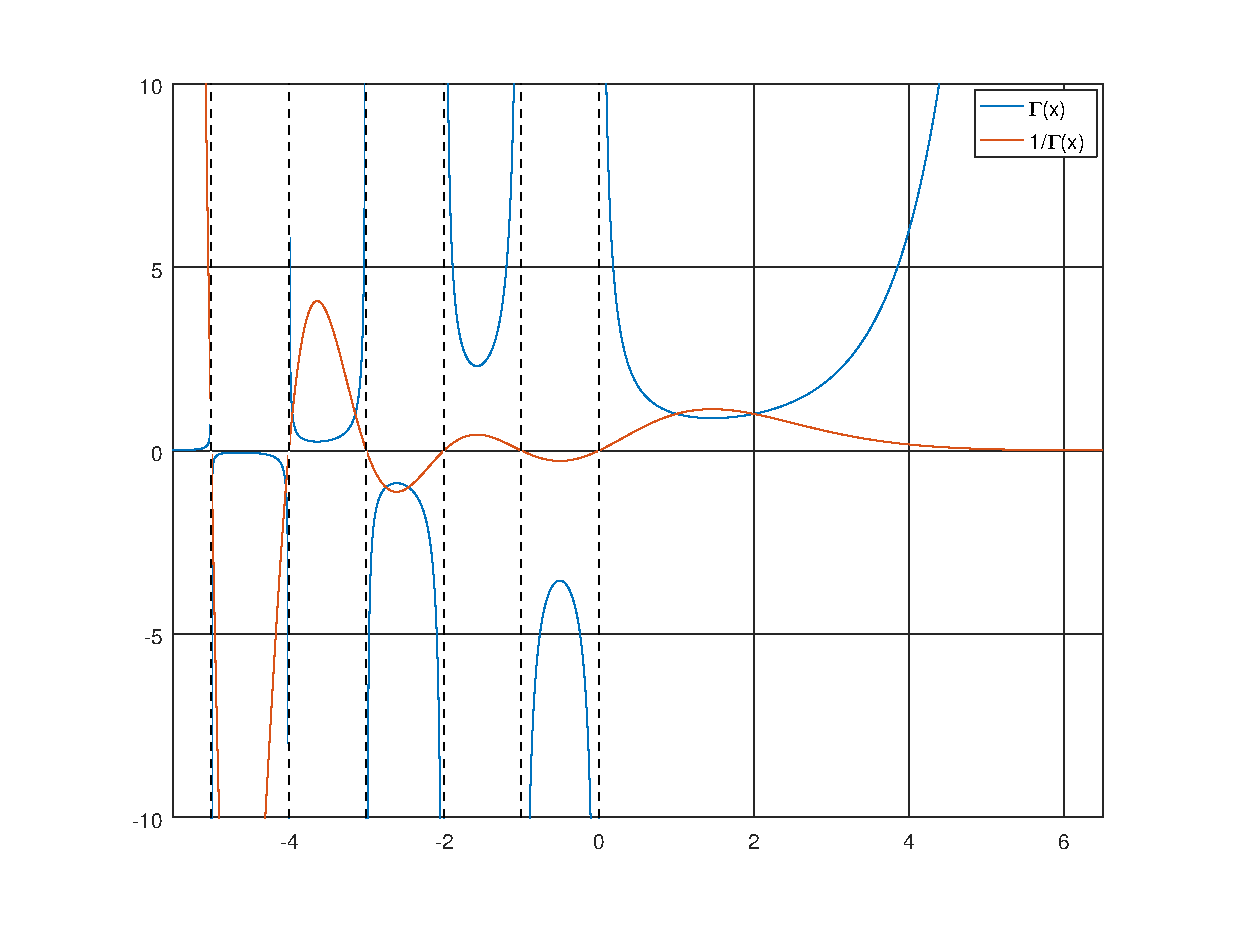
\includegraphics[scale=0.7]{figura1_5.eps}
	\end{center}
\caption{Función gamma y función gamma inversa}
\label{fig1_5}
\end{figure}

Ahora, ¿la función gamma es la única función que genera valores factoriales, satisface la relación de recurrencia y es convexa para $x>0$? Si consideramos la función "pseudo" gamma $\emph{G}_s(x),$ la cual se construye de la siguiente manera 
\begin{align*}
	\emph{G}_s(x) &= 1/x \hspace{1cm}\ &0 < x \leq 1 \\
	\emph{G}_s(x) &= 1				&1 < x \leq 2\\
	\emph{G}_s(x) &= x-1 				&2 < x \leq 3\\
	\emph{G}_s(x) &= (x-1)(x-2)		&3 < x \leq 4\\
	\vdots
\end{align*}
y que está representada en la Figura \ref{fig1_6},
\begin{figure}[htbp]
	\begin{center}
		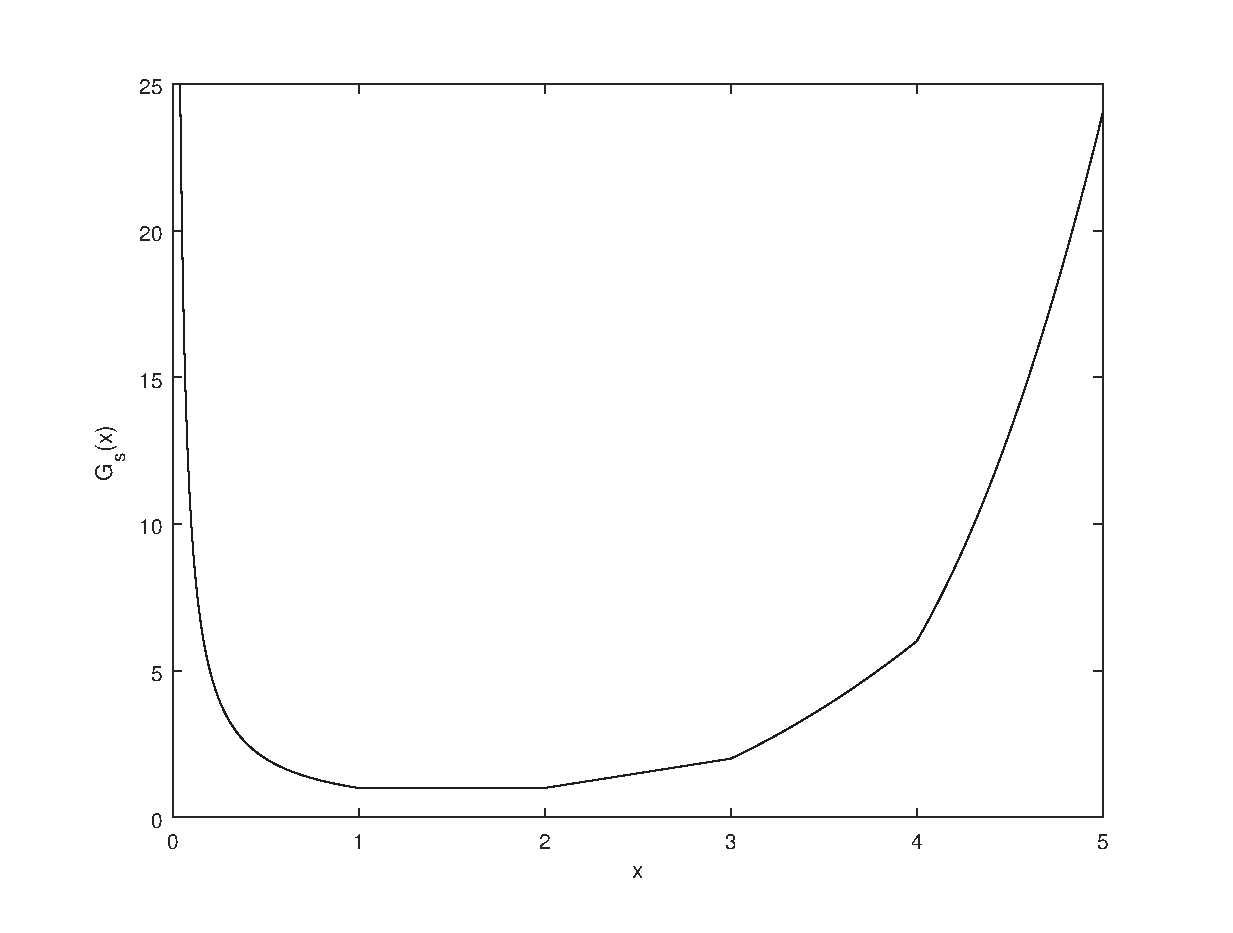
\includegraphics[scale=0.5]{figura1_6.eps}
	\end{center}
\caption{Función pseudogamma}
\label{fig1_6}
\end{figure}
vemos que esta función cumple las condiciones anteriormente discutidas. Se necesita una condición más fuerte, como la de convexidad logarítmica, para poder llegar a caracterizar eficientemente a la función gamma. Podemos ver en la Figura \ref{fig1_7} que la curva del logaritmo de la función gamma es convexa, así, la función gamma es logarítmicamente convexa. En este momento, nos encontramos con el famoso teorema de Bohr-Mollerup, que fue enunciado y demostrado por los matemáticos daneses Harald Bohr (1887-1951) y Johannes Mollerup (1872-1937) en el año 1922. El teorema afirma que la única función que cumple que para $x>0,$ $f(1) = 1,$ sea logarítmicamente convexa y que cumpla con la fórmula de recurrencia $f(x+1) = xf(x),$ es la función gamma de Euler.
\begin{figure}[htbp]
	\begin{center}
		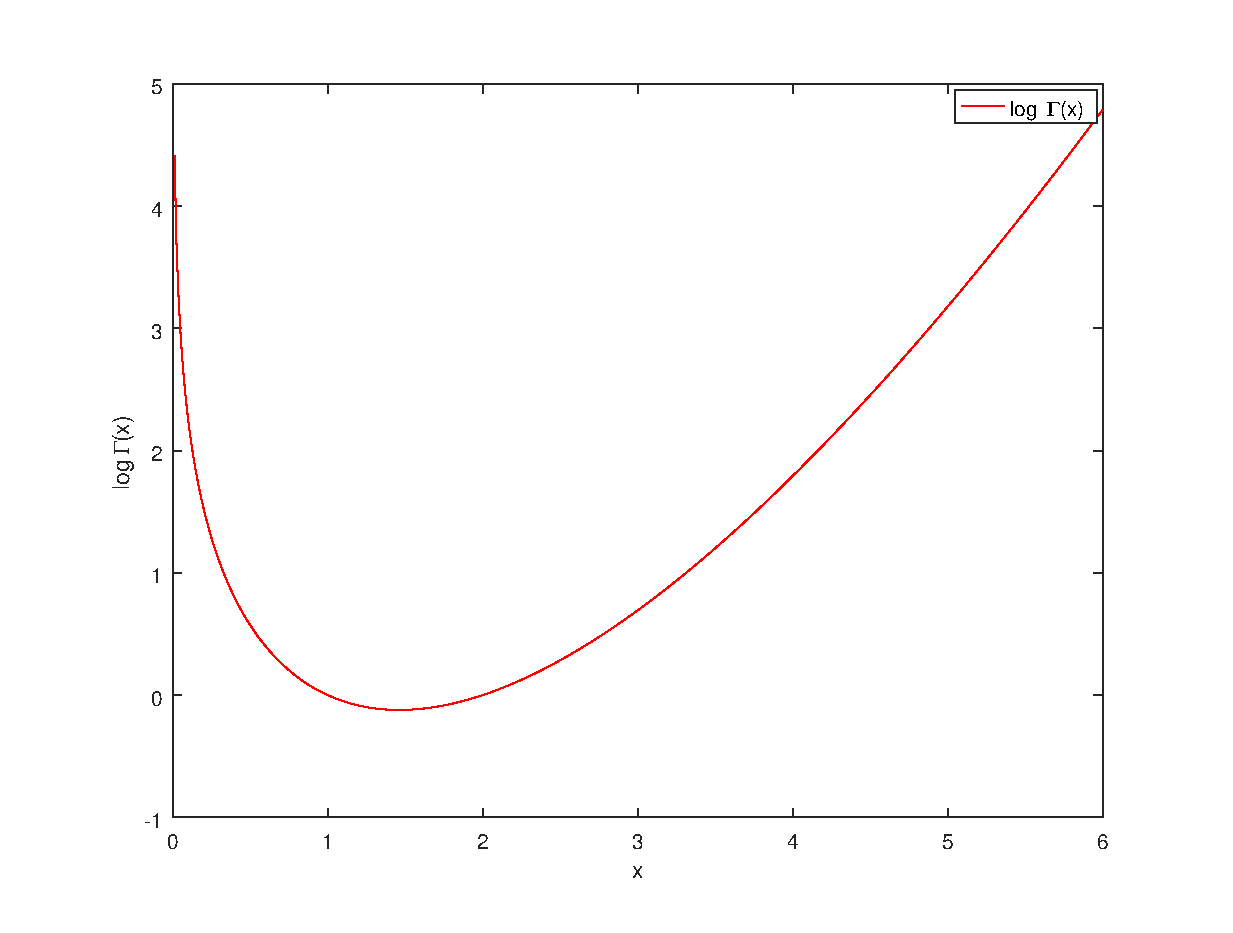
\includegraphics[scale=0.5]{figura1_7.eps}
	\end{center}
\caption{Logaritmo de la función gamma}
\label{fig1_7}
\end{figure}

Para terminar este capítulo, se hace un esbozo muy poco formal del desarrollo de la función gamma hasta la forma integral definida por Legendre. Primero, se parte de la expresión (1.2) y se procede de manera similar a la realizada en Andrews (1999) y Davis (1959). En lo que resta de este capítulo y en el capítulo 2, se necesitan conocimientos de cálculo en la recta real que abarquen convergencia de sucesiones y de series, continuidad, convergencia de sucesiones de funciones, diferenciabilidad e integrabilidad, los cuales Apostol (1967), Arens (2013), Fischer (1983), Little (2015) y Ross (2013) serían de gran utilidad para el lector.

Para $x, n \in \mathbb{Z}_0^+$ con $n>0,$ tenemos que $$(x+n)! = n!\ \prod_{k=1}^{x}(n+k),$$ y además $$(x+n)! = x!\ \prod_{k=1}^{n}(x+k).$$ Por lo anterior, se puede reescribir $x!$ de la siguiente manera
\begin{align*}
	x! &= \frac{x!\prod_{k = 1}^{n}(x+k)}{\prod_{k = 1}^{n}(x+k)} \\
	&= \frac{(x+n)!}{\prod_{k=1}^{n}(x+k)} \\
	&= \frac{n!\ \prod_{k=1}^{x}(n+k)}{\prod_{k=1}^{n}(x+k)} \\
	&= \frac{n!\ n^x}{\prod_{k=1}^{n}(x+k)}\cdot\frac{\prod_{k=1}^{x}(n+k)}{n^x},
\end{align*}
y haciendo $n\rightarrow\infty$, llegamos a que
\begin{align*}
	\lim_{n\rightarrow\infty} x! &= \lim_{n\rightarrow\infty} \left[\frac{n!\  n^x}{\prod_{k=1}^{n}(x+k)}\cdot\frac{\prod_{k=1}^{x}(n+k)}{n^x}\right] \\
	x! &= \lim_{n\rightarrow\infty} \frac{n!\ n^x}{\prod_{k=1}^{n}(x+k)} \cdot \lim_{n\rightarrow\infty} \frac{(n+1)(n+2)\cdot...\cdot(n+x)}{n^x}  \\
	&= \lim_{n\rightarrow\infty} \frac{n!\ n^x}{\prod_{k=1}^{n}(x+k)} \cdot \lim_{n\rightarrow\infty} \left[\left(\frac{n+1}{n}\right)\left(\frac{n+2}{n}\right)\cdot...\cdot\left(\frac{n+x}{n}\right)\right]  \\
	&= \lim_{n\rightarrow\infty} \frac{n!\ n^x}{\prod_{k=1}^{n}(x+k)} \cdot \lim_{n\rightarrow\infty} \left(1+\tfrac{1}{n}\right)\cdot \lim_{n\rightarrow\infty} \left(1+\tfrac{2}{n}\right)\cdot ...\cdot \lim_{n\rightarrow\infty} \left(1+\tfrac{x}{n}\right) \\
	&= \lim_{n\rightarrow\infty} \frac{n!\ n^x}{\prod_{k=1}^{n}(x+k)}.
\end{align*}
Si hacemos $x = 0,$ se obtiene el cociente $n!/n!,$ y así la fórmula se verifica para $x = 0.$ Además, también lo hace para cualquier valor $m \in \mathbb{N},$ aunque no sea muy práctica para hallar tales términos. Veamos, que para $m \in \mathbb{N}$ se tiene que
\begin{align*}
	m! &= \lim_{n \rightarrow \infty} \frac{n!\ n^m}{\prod_{k=1}^{n}(m+k)}\\
		&= \lim_{n \rightarrow \infty} \frac{(\prod_{k=1}^{n}k)\cdot n^m}{\prod_{k=1}^{n}(m+k)}\\
		&= 	\lim_{n \rightarrow \infty} \frac{m!\cdot(\prod_{k=1}^{n-m}(m+k))\cdot n^m}{(\prod_{k=1}^{n-m}(m+k))\cdot(\prod_{k=1}^{m}(n+k))}\\
		&= m!\cdot \lim_{n \rightarrow \infty} \left(\frac{n}{n+1}\cdot\frac{n}{n+2}\cdot\ \dots\ \cdot\frac{n}{n+m}\right)\\
		&= m!
\end{align*}
Ahora, si tomamos $x = 1/2,$ entonces
\begin{align*}
(1/2)! &= \lim_{n \rightarrow \infty}\frac{n!\ \sqrt{n}}{\prod_{k = 1}^{n}\left(\frac{1}{2}+k\right)} \\
&= \lim_{n \rightarrow \infty}\frac{2^n n!\ \sqrt{n}}{\prod_{k = 1}^{n}(2k+1)} \\
&= \lim_{n \rightarrow \infty} \left[\frac{2 \cdot 4 \cdot 6 \cdot 8 \cdot ... \cdot (2n)}{3 \cdot 5 \cdot 7 \cdot 9 \cdot ... \cdot (2n+1)} \sqrt{n}\right] \\
&= \lim_{n \rightarrow \infty}\left[\frac{2 \cdot 4 \cdot 6 \cdot 8 \cdot ... \cdot (2n)}{1 \cdot 3 \cdot 5 \cdot 7 \cdot ... \cdot (2n-1)}\cdot \frac{\sqrt{n}}{(2n+1)}\right], \\
\intertext{y elevando al cuadrado, se obtiene}
[(1/2)!]^2 &= \lim_{n \rightarrow \infty} \left[\frac{2 \cdot 2 \cdot 4 \cdot 4 \cdot 6 \cdot 6 \cdot 8 \cdot 8 \cdot ... \cdot (2n)(2n)}{1 \cdot 1 \cdot 3 \cdot 3 \cdot 5 \cdot 5 \cdot 7 \cdot 7 \cdot ... \cdot (2n-1)(2n-1)}\cdot \frac{n}{(2n+1)^2}\right]  \\
&= \lim_{n \rightarrow \infty} \left[\frac{2 \cdot 2 \cdot 4 \cdot 4 \cdot 6 \cdot 6 \cdot 8 \cdot 8 \cdot ... \cdot (2n)(2n)}{1 \cdot 3 \cdot 3 \cdot 5 \cdot 5 \cdot 7 \cdot 7 \cdot 9 \cdot ... \cdot (2n-1)(2n+1)}\cdot \frac{n}{(2n+1)}\right]  \\
&= \lim_{n \rightarrow \infty} \frac{2 \cdot 2 \cdot 4 \cdot 4 \cdot 6 \cdot 6 \cdot 8 \cdot 8 \cdot ... \cdot (2n)(2n)}{1 \cdot 3 \cdot 3 \cdot 5 \cdot 5 \cdot 7 \cdot 7 \cdot 9 \cdot ... \cdot (2n-1)(2n+1)}\cdot \lim_{n \rightarrow \infty} \frac{n}{(2n+1)} \\
&= \frac{1}{2}\cdot \lim_{n \rightarrow \infty} \frac{2 \cdot 2 \cdot 4 \cdot 4 \cdot 6 \cdot 6 \cdot 8 \cdot 8 \cdot ... \cdot (2n)(2n)}{1 \cdot 3 \cdot 3 \cdot 5 \cdot 5 \cdot 7 \cdot 7 \cdot 9 \cdot ... \cdot (2n-1)(2n+1)} \\
&= \frac{1}{2}\cdot \prod_{k = 1}^{\infty}\ \left(\frac{2k}{2k-1}\cdot\frac{2k}{2k+1}\right).
\end{align*}

El producto infinito resultante se conoce como el producto de Wallis. El matemático inglés John Wallis (1616-1703) descubrió que este producto es igual a $\frac{\pi}{2}$ en el año 1656. A continuación se realiza la deducción de esta fórmula siguiendo la demostración hecha en Hijab (2016).
Vemos que $\forall n\in \mathbb{Z}_0^+$ tal que $n\geq2$ se tiene, $$\int\sin^n x\ dx = \int\sin^{n-1} x \ \sin x \ dx$$
Integrando por partes, se llega a
\begin{equation}
	\int\sin^n x \ dx = -{1 \over n}\sin^{n-1} x \ \cos x +\frac{n-1}{n}\int\sin^{n-2} x \ dx.
\end{equation}
Ahora, evaluando de $0$ a $\pi/2,$ $$\int_{0}^{\pi/2}\sin^n x\ dx = \frac{n-1}{n}\int_{0}^{\pi/2}\sin^{n-2} x \ dx.$$
Como $\int_{0}^{\pi/2} \ dx = {\pi \over 2}$ y $\int_{0}^{\pi/2}\sin x \ dx = 1,$ entonces usando (1.6) para $n\geq2,$ $$\int_{0}^{\pi/2}\sin^2 x \ dx = {1 \over 2}\cdot{\pi \over 2}, \hspace{0.5cm}\int_{0}^{\pi/2}\sin^3 x \ dx = {2 \over 3}\cdot 1,\ \dots$$
Por inducción matemática llegamos a las fórmulas siguientes,
\begin{align*}
	I_{2n} &= \int_{0}^{\pi/2}\sin^{2n} x \ dx = \frac{1}{2}\cdot\frac{3}{4}\cdot\ \dots\ \cdot \frac{2n-3}{2n-2}\cdot\frac{2n-1}{2n}\cdot\frac{\pi}{2}, \ \forall n \in \mathbb{N}\\
	I_{2n+1} &= \int_{0}^{\pi/2}\sin^{2n+1} x \ dx = \frac{2}{3}\cdot\frac{4}{5}\cdot\ \dots\ \cdot \frac{2n-2}{2n-1}\cdot\frac{2n}{2n+1}\cdot 1, \ \forall n \in \mathbb{N}.
\end{align*}
Como $0\leq\sin x \leq1$ en $[0,\pi/2],$ entonces $$0\leq\sin^n x \leq\sin^{n-1} x ,\hspace{0.5 cm}\forall n\geq 1.$$
Además, por propiedad monótona de la integral, $$0 \leq \int_{0}^{\pi/2}\sin^n x \ dx \leq \int_{0}^{\pi/2}\sin^{n-1} x \ dx,\hspace{0.5cm} \forall n\geq 1.$$
Así, $$I_{2n+1}\leq I_{2n}\hspace{0.5cm} \textrm{y} \hspace{0.5cm}I_{2n}\leq I_{2n-1}.$$
Como $$\frac{I_{2n-1}}{I_{2n+1}} = \frac{2n+1}{2n},$$ entonces $$1\leq\frac{I_{2n}}{I_{2n+1}}\leq \frac{I_{2n-1}}{I_{2n+1}} = \frac{2n+1}{2n}.$$
Cuando $n\rightarrow\infty,$ $$\frac{I_{2n}}{I_{2n+1}}\rightarrow\ 1$$ por propiedad de estricción (teorema del emparedado).

Además, tenemos que $$\frac{I_{2n+1}}{I_{2n}} = \frac{2}{\pi}\cdot\frac{2\cdot2\cdot4\cdot4\cdot\ \dots\ \cdot(2n-2)(2n-2)(2n)(2n)}{1\cdot3\cdot3\cdot5\cdot\ \dots\ \cdot(2n-3)(2n-1)(2n-1)(2n+1)},$$ entonces
$$\frac{\pi}{2} = \frac{I_{2n}}{I_{2n+1}}\cdot\frac{2\cdot2\cdot4\cdot4\cdot\ \dots\ \cdot(2n-2)(2n-2)(2n)(2n)}{1\cdot3\cdot3\cdot5\cdot\ \dots\ \cdot(2n-3)(2n-1)(2n-1)(2n+1)}$$ y haciendo $n\rightarrow\infty$ llegamos al siguiente resultado $$\lim_{n \rightarrow \infty}\ \frac{2\cdot2\cdot4\cdot4\cdot\ \dots\ \cdot(2n)(2n)}{1\cdot3\cdot3\cdot5\cdot\ \dots\ \cdot(2n-1)(2n+1)} = \frac{\pi}{2},$$ que en otras palabras es $$\prod_{k = 1}^{\infty}\ \left(\frac{2k}{2k-1}\cdot\frac{2k}{2k+1}\right) = \frac{\pi}{2}.$$ Por lo anterior  $$\left({1 \over 2}\right)! = {\sqrt{\pi}\over 2},$$ 
así que la expresión (1.4) es válida, en lo que respecta al tratamiento heurístico que se está abordando.
 
Por último, se deduce (1.3) a partir de la integral de Euler de primera especie, tomando como base a Euler (1738) y a Andrews (1999). Luego, llegamos a la representación de Legendre siguiendo a Andrews (1999) y a Davis (1959). Pero antes de realizar tal procedimiento preguntémonos, ¿por qué la integral de Euler de primera especie? Aunque Euler no lo mencionó de manera explícita, el hecho de que $(1/2)! = \sqrt{\pi}/2$ pudo haberlo animado a usar la integral $$\int_{0}^{1}\sqrt{1-x^2}\ dx = \int_{0}^{1}(1+x)^{1/2}\ (1-x)^{1/2}\ dx = \frac{\pi}{4},$$ la cual representa el área de la cuarta parte del círculo unitario. Vemos que tal expresión posee alguna similitud con la integral de primera especie, donde $n = 1/2$ arroja una pista para la deducción de la integral de segunda especie.

Así, usando el teorema del binomio de Newton con $n \in \mathbb{Z}_0^+$ en la integral de Euler de primera especie $$\int_{0}^{1}x^m\ (1-x)^n\ dx,$$ obtenemos
\begin{align*}
	\int_{0}^{1} x^m\ (1-x)^n\ dx = \sum_{k = 0}^{n}\binom{n}{k}(-1)^k\frac{1}{m+k+1}.
\end{align*}
Por consiguiente, para $n = 0$ llegamos a $$\int_{0}^{1}x^m\ dx = \frac{1}{m+1},$$
para $n = 1$
$$\int_{0}^{1}x^m\ (1-x)\ dx = \frac{1}{m+1} - \frac{1}{m+2} = \frac{1}{(m+1)(m+2)},$$
para $n = 2$
$$\int_{0}^{1}x^m\ (1-x)^2\ dx = \frac{1}{m+1} - \frac{2}{m+2} + \frac{1}{m+3} = \frac{1 \cdot 2}{(m+1)(m+2)(m+3)},$$
y así por inducción matemática, usando integración por partes, obtenemos la expresión $$\int_{0}^{1}x^m\ (1-x)^n\ dx = \frac{n!}{(m+1)(m+2)(m+3) \cdot \ldots \cdot (m+n+1)},$$ para $n \in \mathbb{Z}_0^+.$

Si $m = f/g,$ donde $f,g \in \mathbb{Z}_0^+$ con $g \neq 0,$ entonces
$$\frac{n!}{(f+g)(f+2g) \cdot \ldots \cdot (f+ng)} = \frac{f+(n+1)g}{g^{n+1}}\int_{0}^{1}x^{f/g}(1-x)^n\ dx,$$ haciendo $x = t^{\frac{g}{f+g}}$ tenemos que
$$\frac{n!}{(f+g)(f+2g) \cdot \ldots \cdot (f+ng)} = \frac{f+(n+1)g}{(f+g)^{n+1}}\int_{0}^{1}\left(\frac{1-t^{\frac{g}{f+g}}}{\tfrac{g}{f+g}}\right)^n\ dt.$$ Si $f = 1$ y $g = 0,$ entonces $k = \frac{g}{f+g} = 0,$ usando la regla de l'Hôpital llegamos a $$\lim_{k \rightarrow 0} \frac{1-t^k}{k} = -\ln t,$$ y así
$$n! = \int_{0}^{1}\ (-\ln t)^n\ dt.$$

La integral de Euler es válida para todo número positivo, y en el momento fue conocida como la integral de Euler de segunda especie, Davis (1959). Legendre, partiendo de la expresión $$(n-1)! = \int_{0}^{1}\ (-\ln x)^{n-1}\ dx,$$ dedujo lo que hoy se conoce como la función gamma de Euler por medio del cambio de variable $$t = -\ln x.$$ Como la función $\ln$ es creciente, entonces
$$(n-1)! = \int_{\infty}^{0}\ t^{n-1}\ (-x)\ dt = \int_{0}^{\infty}\ t^{n-1}\ x\ dt,$$ y utilizando el cambio de variable, donde $x = e^{-t},$ obtenemos $$(n-1)! = \int_{0}^{\infty}\ t^{n-1}\ e^{-t}\ dt.$$ Finalmente, llegamos a la representación clásica de la función gamma de Euler, definida por Legendre de la siguiente manera, $$\Gamma (x) = \int_{0}^{\infty}\  e^{-t}\ t^{x-1}\ dt,\ \textrm{para}\ x \in \mathbb{R}_{>0}.$$
\endinput